%%% Clinic Statement of Work Template
%%%
%%% C.M. Connelly <cmc@math.hmc.edu>
%%%
%%%  $Id: statement-of-work-template.tex 251 2007-09-17 18:41:19Z cmc $

%%% Copyright (C) 2004-2007 Claire M. Connelly and 
%%% the Department of Mathematics, Harvey Mudd College.
%%%
%%% This file is part of the hmcclinic class document provided to
%%% HMC mathematics students.
%%%
%%% Modified for cguclinic class.
%%%
%%% See the COPYING document, which should accompany this
%%% distribution, for information about distribution and
%%% modification of the document and its components.


%%% Clinic reports use the clinic class, which should be located
%%% somewhere in TeX's search path

%%% For your ``statement of work'' (or ``work statement''), specify
%%% the ``proposal'' document-class option to the hmcclinic class.
\documentclass[proposal]{cguclinic}
%\usepackage{subcaption,circuitikz,tikz}
\usepackage{float}

%%% The major difference between the statement of work and a midyear
%%% or final report is that the statement of work is typeset as an
%%% article, which means that the highest level of structural
%%% division available to you is section rather than chapter.

%%% There are also some changes in pagination styles and content
%%% that reflect the briefer nature of the proposal.  For example,
%%% in the longer reports, you use \frontmatter, \mainmatter, and
%%% \backmatter to separate some sections of the report from
%%% others.  In the statement of work, you don't need those
%%% commands, as no such division is necessary.

%%% Other packages needed by your document may be loaded here.
% \usepackage{url}              % For formatting URLs and other web or
                                % file references.

%%% Provide additional context around errors. 
\setcounter{errorcontextlines}{1000}


%%% Information about this document.

%%% I find it most useful to put identifying information about a
%%% document near the top of the preamble.  Technically, this
%%% information must precede the \maketitle command, which often
%%% appears immediately after the beginning of the document 
%%% environment.  Placing it near the top of the document makes it
%%% easier to identify the document, and keeps it out from getting
%%% mixed up with the real meat of the document.

%%% We use the same set of commands for specifying information about
%%% the people involved with the project that are used in the longer
%%% reports, so you can copy most of this information directly into
%%% your midyear and final reports.

%%% So, some questions.

%% What is the name of the company or organization sponsoring your project?
\sponsor{Sandia National Laboratories}

%% What is the title of your report?
\title{Graph Theoretic Machine Learning Approaches to Predict Atomic Scale Fracture in Silica-Based Glasses}

%% Who are the authors of the report (your team members)?  (Separate
%% names with \and.)
\author{Shu Cheng \and Yuri Kim \and Adam Lawrence (Project Manager) \and Corina Oroz}

%% What is your faculty advisor's name?  (Again, separate names with
%% \and, if necessary.)
\advisor{Allon Percus}

%% Liaison's name or names?
\liaison{Mark Wilson \and Thomas Hardin }

%% Did you have an outside consultant help you with this project?  Put
%% their names in the \consultant command.
%\consultant{Joseph Jones}

% \date{}
% Uncomment to manually edit date. Commented, TeX will automatically insert today's date.

%%% End of information section.

%%% New commands and environments.

%%% You can define your own commands and environments here.  If you
%%% have a lot of material here, you might want to consider splitting
%%% the commands and environments into a separate ``style'' file that
%%% you load with \usepackage.

%\newcommand{\coolcommand}[1]{#1 is cool.} % Lets everyone know that
                                % the person or thing that you provide
                                % as the argument to the command is
                                % cool.


%%% Some theorem-like command definitions.

%%% The \newtheorem command comes from the amsthm package.  That
%%% package is loaded by the class file.

%%% Note that these definitions have changed from the version in the
%%% sample report document by dropping the ``within'' argument.  See
%%% Gratzer's _Math into LaTeX_ or the AMS-LaTeX documentation for
%%% more details.

% \newtheorem{thm}{Theorem}
% \newtheorem{Theo1}{Theorem}
% \newtheorem{Theo2}{Theorem}
% \newtheorem{Lemma}{Lemma}
\usepackage{url}
\usepackage{amsmath}
\usepackage{tikz}
\usetikzlibrary{shapes,arrows}

\usepackage{comment}




\usepackage{graphicx}


 

%%% If you find that some words in your document are being hyphenated
%%% incorrectly, you can specify the correct hyphenation using the
%%% \hyphenation command.  Note that words are separated by
%%% whitespace, as shown below.

%\hyphenation{ap-pen-dix wer-ther-i-an}


%%% The start of the document!

%% The document environment is the main environment in any LaTeX
%% document.  It contains other environments, as well as your text.

\begin{document}

%%% In a longer document (such as your midterm and final reports),
%%% you would have separate \frontmatter, \mainmatter, and
%%% \backmatter commands to define some large chunks of your
%%% document.  For the Statement of Work, which is a short document,
%%% we don't need these commands.

%%% Your Statement of Work begins with a title page.  The title page
%%% is formatted by commands in the document class file, so you
%%% don't need to worry about what it looks like -- just putting the
%%% \maketitle command in your document (and filling in the necessary
%%% information for the identification commands above) is enough.
\maketitle

%%% In a longer document or an article being submitted to a journal
%%% or conference, you would probably have an abstract that
%%% summarized the purpose of the document.  We don't need that for
%%% a Statement of Work.

%%% Similarly, in longer documents you would probably have commands
%%% to include a table of contents and lists of figures or tables.
%%% For a short document such as the Statement of Work, we don't
%%% need these commands.


%%% Content.

%%% For smaller documents---especially those you're writing by
%%% yourself---you might write your entire report using a single LaTeX
%%% source file.  For larger documents, we recommend that you split
%%% the source file into several separate, smaller files.  The smaller
%%% files are ``included'' into your main, or ``master'' document
%%% using \include commands.  See the template file for the Clinic
%%% reports for more details on how to split a LaTeX project into
%%% smaller files.


%%% The body of your Statement of Work should appear here.  See
%%% Chapter 4 in _The Mathematics Clinic in Brief: A Handbook_ for
%%% more details on what you should include in a Statement of Work.

\pretolerance=3000

\section{Abstract}
\label{sec: Abstract}

$\indent$ Predicting where the failure in a brittle material occurs plays a critical role in many engineering topics. These brittle materials are prevalent in many indsutrial applications. The primary challenge in these studies is not only locating the nucleation of a fracture but making realistic lifespan prediction on how fractures propagate. 

 Currently, molecular dynamic simulations are the only way to incorporate the effects of chemistry in fracture modeling. Researchers at Sandia National Laboratories have been exploring new methods to supplement the current methods to improve computational efficiency as well as prediction accuracy. 

The Clinic team aims to incorporate a graph theoretic approach based on labeled MD simulated silica-based glasses in order to accurately and predict fracture nucleation and propagation. Environmental and chemical considerations will be taken into account and supervised machine learning methods will be used to create a surrogate model that can validate on existing simulation results. 


 
 
 %Graph network machine learning structures may become effective tools in  computational molecular dynamics %(MD). Already, there have been techniques developed using topological constraints based on features such as %atomic flexibility and internal stress of materials to predict their chemical reactivity and composition %\cite{bauchy}. This project will explore and outline a novel approach to predicting fracture nucleation and %fracture propagation in silicate glasses using a graph network to study local structure of silicate atoms.
 
 %The clinic team will address the problem of predicting fracture propagation and nucleation in MD simulated
%silica-based glasses in environmental conditions with local atomic structure. A graph theoretical approach
%%will be used to create a surrogate model, based on supervised learning techniques that are trained on MD
%data, to provide a rapid prediction of the fully atomistic simulation. These predictions will then be correlated
%back to atomic structure, and validated on existing large-scale atomic MD simulation results.

\section{Background}
\label{sec: Background}
% This is the project description we were provided we can tailor it later
Silicate glasses are very important materials in fields including medicine, optics, electronics, telecommunication and energy.  Figure \ref{crack_prop} shows a 3D visualization of this simulation with perspective. Given that glass is extremely brittle, fractures may occur instantaneously when a maximum stress level is reached.
\bigskip
%%  CRACK PROPEGATION SIMULATION FIGURE 
\begin{figure}
    \centering
    \noindent
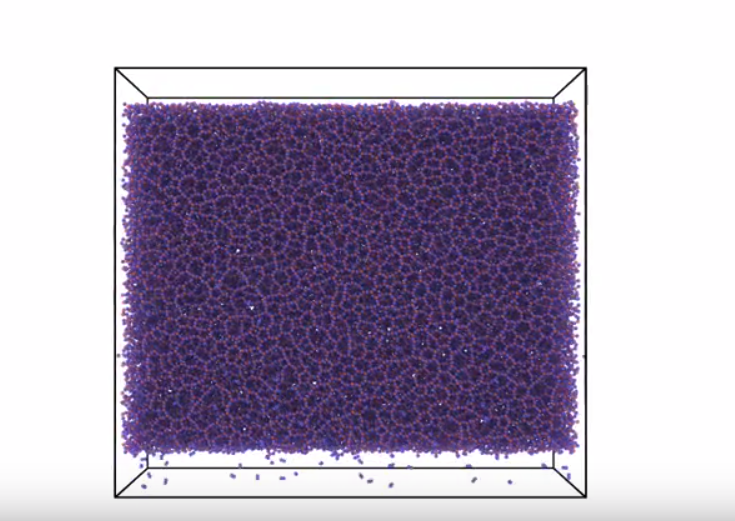
\includegraphics[width=0.4\textwidth]{picture/frac_prop1.PNG}\hspace{0.2\textwidth}%
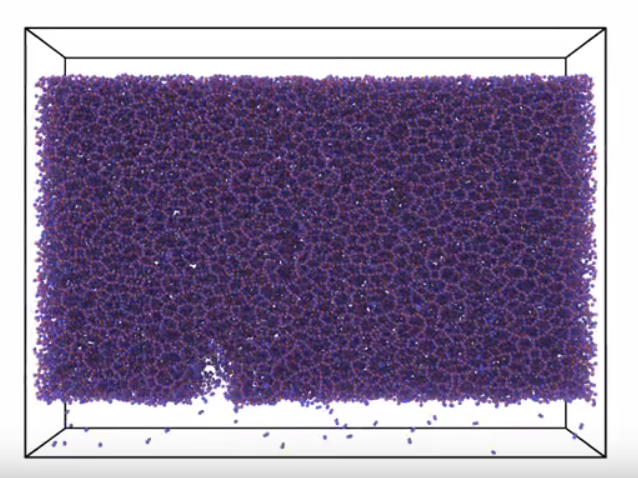
\includegraphics[width=0.4\textwidth]{picture/frac_prop2.PNG}\\[2em]
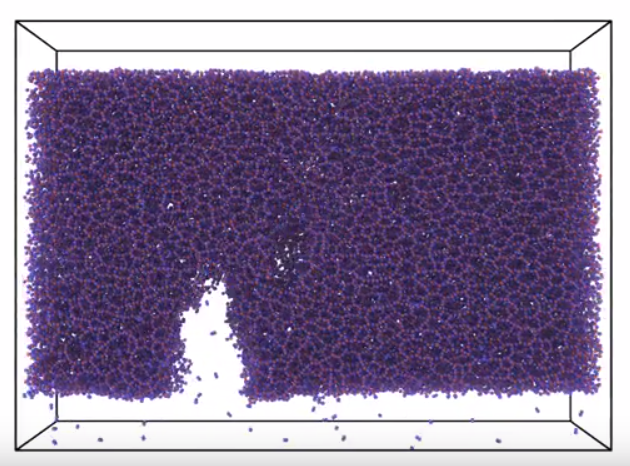
\includegraphics[width=0.4\textwidth]{picture/frac_prop3.PNG}\hspace{0.2\textwidth}%
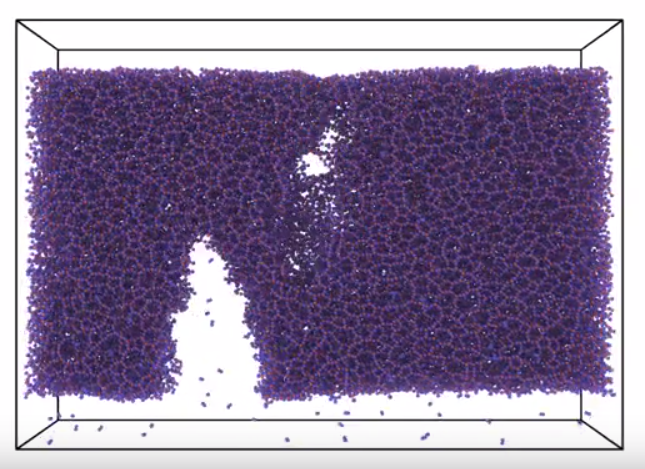
\includegraphics[width=0.4\textwidth]{picture/frac_prop4.PNG}\par
    \caption{Crack propagation}
    \label{crack_prop}
\end{figure}
%%%%%%%%%%%%%%%%%%%%%%%%%%%%%%%%%%%%%%%

Typically in these silicate glass structures, silicon (Si) is surrounded by four oxygen (O) atoms forming a tetrahedron seen in Figure *Figure being created*. These tetrahedra share one common O atom if they are neighbors. A ring forms if a group of tetrahedra share common O atoms, and the size of these rings is computed based on how many Si atoms are in the ring. A large ring has 11 and 12 Si atoms, medium rings have 5 and 6, and small rings have 1 or 2. An atom is denoted as under-coordinated if the number of its constraints is lower than 4, and over-constrained, if greater than 4. \cite{pedone2015dynamics}

It was also shown that increasing the quenching rates, increased the number of large-sized rings and decreased the number of medium-sized rings decreases. The change in the number of small-sized rings was minimal. And because there is larger void in large-sized ring, it can be stretched and deformed more than the medium-sized ring. However, medium-sized ring can take more per unit stress while tensile is applied, so it has more strain energy.

Classical molecular dynamics simulations were also used to investigate the properties of silicate glasses. Glasses were observed using 60k atoms for soda-silicate glasses and 30k atoms for silica glass . Soda-lime silicate glasses were analyzed at the nanometric scale with an atomic force microscope. Cavities were formed at 20nm long and 5nm deep ahead of the crack tip, and cracks would advance following the coalescence of cavities .

Regarding the mechanical properties of the silicate glass, Young's modulus, strength, failure strain and fracture mechanism were all used throughout the study.  Additionally, these properties depend on both the strain rate and the quench rate. The glasses were heated at 5000 K, a temperature considered more than adequate to bring the glass into a liquid state and the heat was equilibrated for 100 picoseconds and then cooled continuously to 300 K with a normal cooling rate of 5 K/ps. .

With regards to stress, uniaxial tensile tests were implemented along the z-axis for both bulk glasses and nanowires. An important finding is such that for uniaxial tension tests in bulk glasses, in particular flaw-free silica glass, the glass was forced to break in a brittle manner. Additionally, in flaw-free glass, voids would grow, then coalesce before the structure would fracture. What was concluded as a result of the numerous tests performed was that the fracture mechanism of defective models showed to be less brittle compared to flaw-free glass given the unstable region is capable of expansion . This is an important finding given that it contradicts what is generally expected of silicate glasses.\cite{radialDistribution}

Nucleation of fractures originates from defects of the atomic structure of silicate glass. 
The fractures do not necessarily occur when the weakest bond in the structure breaks and triggers numerous other breaks in the surrounding bonds. Instead, the fracturing is dependent on the local structure surrounding the atoms so defining this relation is critical in the fracture analysis. While these relations can be studied using results from MD, a repetitive simulation-observation approach is computationally prohibitive. A more tractable approach is to use machine learning and surrogate modeling techniques.

Molecular dynamics (MD) simulations have shown that silicates that have their fracture regions contacted with an aqueous environment have their Si-O bond energy threshold lowered by 25$\%$  \cite{chem_effects}. Since there is both mechanical loading (stress) and chemical that affect the crack tips, it becomes more difficult to predict fracture propagation. Running simulations of the chemical-mechanical effects on crack tips showed differing rates of fracture propagation as well as changes in fracture direction and even stress distribution in the atoms in the fracture process zone. 

Therefore, knowing the initial conditions of the silicate glass environment is critical in predicting fracture behavior and  will test the robustness of our model.


%% ANOTHER PICTURE 
%\begin{figure}[!b]
%  \centering
%  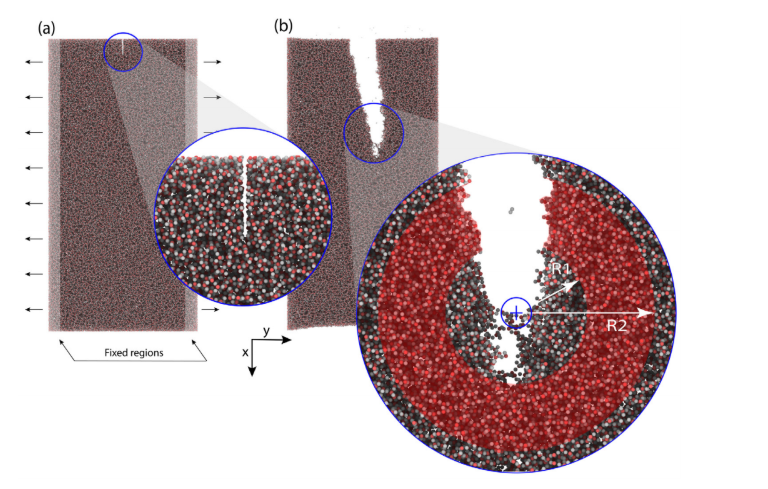
\includegraphics[width=11cm]{picture/FractureMechanism.PNG}
%  \caption{Images of a simulated a-SiO2 sample. (a) Samples are loaded and held in mode I tension. Initial %cracks are created by removing a
%small number of atoms from the upper surface of the sample. (b) An example of crack propagation in a %loaded sample, with the crack tip
%identified by the +, and the annulus colored red. Figure reproduced %from~\protect\cite{mWilson_continuum_stress}} 
%  \label{crack_prop2}
%\end{figure}


%% EL NUMERO TRES 
%\begin{figure}[!h]
%  \centering
%  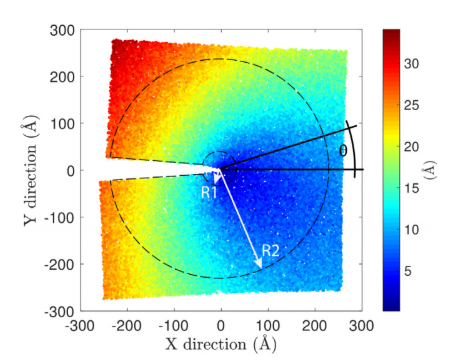
\includegraphics[width=11cm]{picture/FractureMechanism2.PNG}
%  \caption{Configuration showing the coordinate axes and crack tip relationship similar to the Williams %expansion. Dashed lines show an annulus
%with inner radius R1 and outer R2. Points are colored according to the magnitude of their displacement %%under an applied field. Figure reproduced from~\protect\cite{mWilson_continuum_stress}} 
 % \label{crack_rad2}
%\end{figure}

\section{Goals}
\label{sec: Goals}
In this project, our ultimate goal is using machine learning methods to learn from Molecular Dynamics simulations, so that the trained machine learning models can produce rapid predictions of simulation results without the extensive computation that simulations would take. To realize the ultimate goal, we separate it into two sub-goals. One of the sub-goals is to predict fracture nucleation and the other one is to predict fracture propagation. The nucleation event is where fractures will emerge and must be predicted in a certain region and fracture propagation is a continuing process of atoms being included in the fracture region, also known as the process zone. And we will use two different models to address these problems respectively. 



\begin{itemize}
\item \textbf{Goal 1:} \emph{Predicting Fracture Nucleation Events} 
\begin{itemize} 
    \item Definition of fracture nucleation: Nucleation event is the creation of void in the material. As stress is applied uni-axially, bonds break and form among atoms. Correspondingly, some atoms have growing void among themselves and others are squished into a more dense region. And fracture nucleates alongside the void occurrence. 
    
    As a result, we define that whether an atom/a node is part of a nucleation event, using a local density measure, which is the Voronoi cell volume $v_i$, around a certain atom $i$. It is a volume measure because we are measuring the volume around the atom in a 3D graph. 
    So, if $v_i$ exceeds a certain threshold, then atom $i$ is defined as part of a nucleation event. In this project, we set the threshold to be 3 standard deviation from the mean value, $\mu_v$, at the current time step.
    \textbf{1. Could insert a figure here demonstrating 3D Voronoi volume}
    \textbf{2. Could insert 3 figures demonstrating why we choose 3sd as our threshold}
    \[
    nuc_v = \frac{(v_i - \mu_v)}{\sigma_v}
    \]  
    \item Contrary to a fracture propagation event, where there is existing void, and fracture just keeps growing along the existing fracture, a nucleation event has no existing fracture to propagates along. As a result, it is different to predict nucleation event. We assume that a nucleation event is primarily influenced by the local structure at the atomic level of the material. And a Recurrent Neural Network model is built to identify these latent structures. Detailed explanation is presented in the method section.
    
\end{itemize}
\end{itemize}


\begin{itemize}
\item \textbf{Goal 2:} \emph{Predicting Fracture Propagation} 
\begin{itemize} 
    \item Definition of fracture in a dynamic setting:
    
    \item Method: We are going to use a derivation of recurrent neural network(RNN), the long-short term memory networks(LSTM) to predict the propagation of an existing interstices. The reason why we choose LSTM over RNN is that it's a more flexible model and can control how much of a memory we would like the model to contain when making predictions.
    
    
    
    
    
\end{itemize}



\end{itemize}


%\section{Data}
%\label{sec: Data}
%The training data consists of one hundred silicate samples with the following setup: 
\begin{enumerate}
    \item Dry (vacuum), free surfaces in two directions.
    \item Wet (H20 in voids), free surfaces in two directions
    \item Dry (vacuum), fully periodic (toroidal) boundary conditions.
    \item Wet (H20 in voids), fully periodic (toroidal) boundary conditions.
\end{enumerate}

The silicate is exposed to these conditions following uniform quenching process done at 3.7K/picoseconds. So although we have four different environmental conditions, the procedures starts at equilibrium.
Each instance will contain snapshots of the atoms through time as well as information regarding charge, stress tensor and bond connectivity. 

Molecular dynamics (MD) simulations have shown that silicates that have their fracture regions contacted with an aqueous environment have their Si-O bond energy threshold lowered by 25$\%$  \cite{chem_effects}. Since there are?is? both mechanical loading (stress) and chemical that affect the crack tips, it becomes more difficult to predict fracture propagation. Running simulations of the chemical-mechanical effects on crack tips showed differing rates of fracture propagation as well as changes in fracture direction and even stress distribution in the atoms in the fracture process zone. 

\begin{comment}
\begin{figure}[!b]
  \centering
  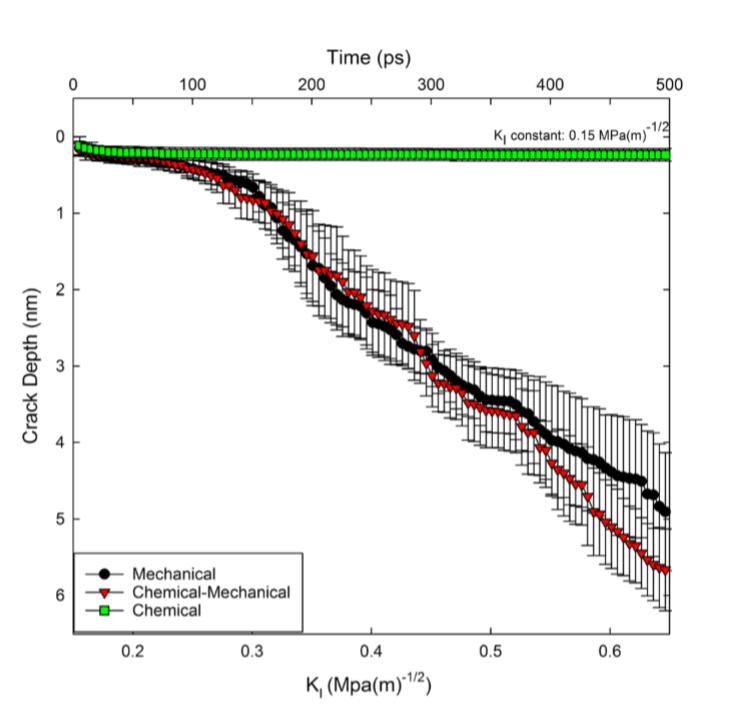
\includegraphics[width=11cm]{picture/crack_depth.PNG}
  \caption{Crack depth for silica systems under mechanical, chemical, and chemical-mechanical conditions.  Figure reproduced from~\protect\cite{chem_effects}}
  \label{crack_depth}
\end{figure}
\end{comment}

\begin{comment}
\begin{figure}[!b]
  \centering
  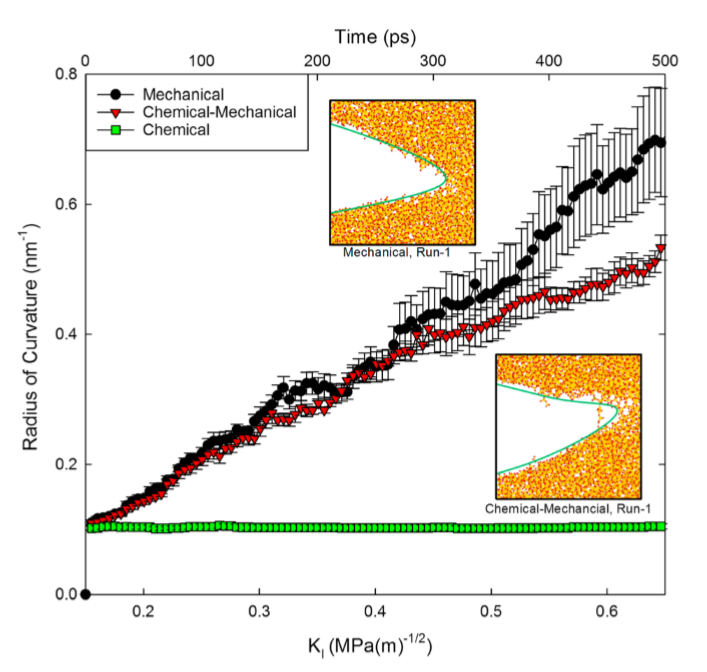
\includegraphics[width=11cm]{picture/crack_radius.PNG}
  \caption{Radius of curavture for silica systems under mechanical, chemical, and chemical-mechanical conditions. Figure reproduced from~\protect\cite{chem_effects}} 
  \label{crack_rad}
\end{figure}
\end{comment}

Therefore, knowing the initial conditions of the silicate glass environment is critical in predicting fracture behavior and  will test the robustness of our model.

\begin{comment}
\begin{figure}[ht]
    \centering
    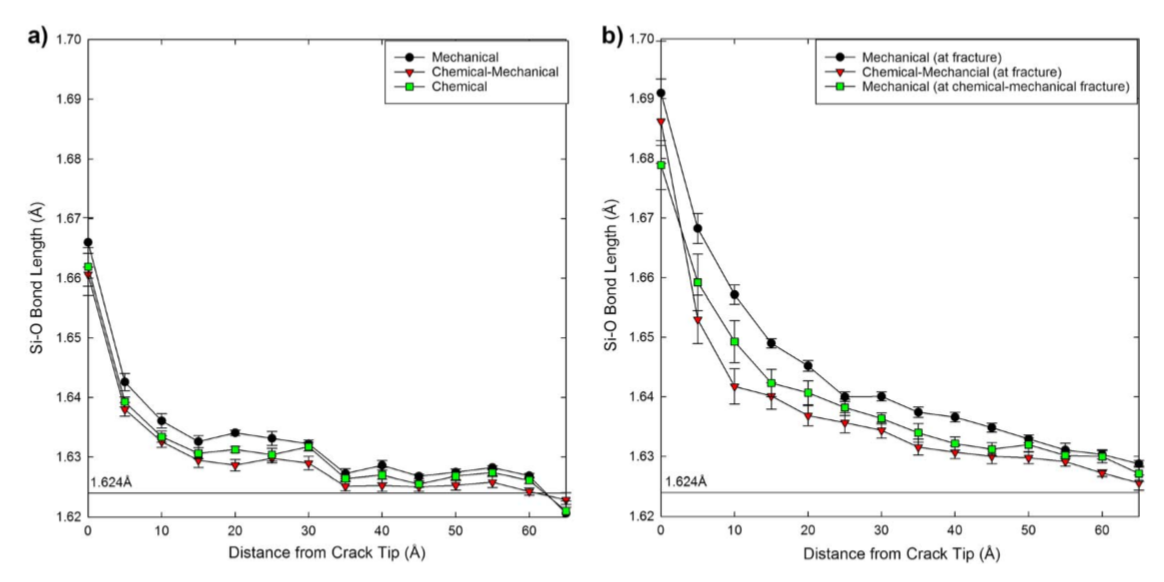
\includegraphics[width=10cm]{picture/AverageSiO.PNG}
    \caption{Average Si─O bond length based on distance from the crack tip at (a) initial conditions and (b) after loading.}
    \label{Average Si-O}
\end{figure}
\end{comment}




\section{Methods}
\label{sec: Methods}
Below are the list of methods we will be using to solve the project goals.

\begin{itemize}

\item \textbf{Graph Representation}
\bigskip
In order to be able to predict the atomic scale fracture nucleation and propagation in silica-based glasses, we must first find an appropriate mathematical graph representation. 
\begin{itemize}
    \item \textbf{Basic Graph Representation}
    \\
    The most basic way to define a graph is naive. In one sample, we have a total number of $n$ atoms. An atom, either a Silicon atom or an Oxygen atom, is defined as a vertex $v_i$, where $0 \leq i \leq n$ and a set of such vertices is $\mathbf{V} = \{v_0,v_1,...v_{n-1}\}$. An edge, $e_i$ is defined as a mechanical trusses between two atoms. A set of such edges is $\mathbf{E} = \{e_0,e_1,...e_{n-1}\}$. As uni-axial stress is applied to the material, edges could break and form between any two vertices, where state 1 means an edge is broken and state 0 means an edge exists. Therefore, an set of active edges, defined as $\mathbf{E_a}$, includes all the edges that have broke or formed at least once, meaning they have changed their state, either from 1 to 0 or from 0 to 1 at one point. As a result, the graph \textbf{G} is thus defined as a discrete set of vertices \textit{V} connected by a set of edges \textit{E}. We can denote it as $\ G = (V,E)$, where the size of the graph is $\ |V| = n $.
    
    \item \textbf{Reduced Graph Representation}
    \\
    
    
\end{itemize}


\item \textbf{Feature Description}
\bigskip

To use ML algorithms, we want to characterize vertices based on features such as charge, stress tensor, type and centrality.

\begin{itemize}
    \item \textbf{Centrality:} In graph theory, centrality is use to identify the most important vertices. An example could be a specific silicon atom that is at the center of where a fracture nucleates. Identifying these vertices with the most centrality will allow us to predict fracture
\end{itemize}







\\

\item \textbf{Machine Learning Methods}
\bigskip
\\


\textit{Below are old stuff}
\item \textbf{Method for Identifying Fracture Nucleation} 
\bigskip
\\

Lets construct our own simple graph. 
\bigskip
\\
% CONSTRUCTION OF EXAMPLE GRAPH SiO3 %%%%%%%%%%%%%%%%%%%%%%%%%%%%%%%%%%%%%%%%%%%%%%%%%%%%%%%%%%%%%%%%%%%%
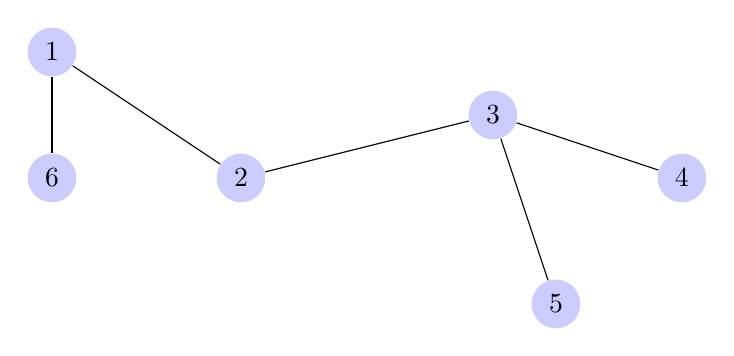
\begin{tikzpicture}
  [scale=.8,auto=left,every node/.style={circle,fill=blue!20}]
  \node (n6) at (1,10) {1};
  \node (n4) at (4,8)  {2};
  \node (n5) at (8,9)  {3};
  \node (n1) at (11,8) {4};
  \node (n2) at (9,6)  {5};
  \node (n7) at (1,8)  {6};

  \foreach \from/\to in {n6/n4,n4/n5,n5/n1,n2/n5,n6/n7}
    \draw (\from) -- (\to);

\end{tikzpicture}
%%%%%%%%%%%%%%%%%%%%%%%%%%%%%%%%%%%%%%%%%%%%%%%%%%%%%%%%%%%%%%%%%%%%%%%%%%%%%%%%%%%%%%%%%%%%%%%%%%%%%%%%%%
\bigskip
\\
% THIS IS PRETTY WONKY NOTATION MAYBE A BETTER WAY OF LABLING ??

Graphs hold many properties that will motivate and guide our research. First we can consider the \textbf{degree} of a vertex. Denoted $\deg(v_{i})$ the degree is the number of edges connected with the vertex.For example node 3, Si has $\deg(v_{3}) = 3$. 
\bigskip
\\
Since we will be working with a large data set of vertices, we can store degree information for each vertex in a \textbf{degree matrix}. Given a graph $\ G(V,E)$ where \textit{n} is the number of nodes, the degree matrix of G is a diagonal matrix who's entries are the degree of each vertex. 
\bigskip
\\
The degree matrix for our graph would be the following. 
$$
\begin{vmatrix}
2&0&0&0&0&0\\
0&2&0&0&0&0\\
0&0&3&0&0&0\\
0&0&0&1&0&0\\
0&0&0&0&1&0\\
0&0&0&0&0&1\\
\end{vmatrix}
$$
\\
Notice the degree matrix of a graph is \textit{always} diagonal. 
\bigskip
\\
Another matrix we need to consider for storing our graph information is called the \textbf{adjaceny matrix}. Adjacency matrix denoted $\ A_{i,j}$ is exactly what is sounds like. If there exists an edge between two nodes then $\ A_{i,j} = 1$ , else 0. For our graph above the adjacency matrix will be:
\\
$$
\begin{vmatrix}
0&1&0&0&0&1\\
1&0&1&0&0&0\\
0&1&0&1&1&0\\
0&0&1&0&0&0\\
0&0&1&0&0&0\\
1&0&0&0&0&0\\
\end{vmatrix}
$$
\\
Note that all undirected graphs are symmetric. 
\bigskip
\\
Perhaps one of the most useful data structure used our graph representation will be the \textbf{Laplacian Matrix}. Simply put the Laplacian matrix is \textbf{D} - \textbf{A}. Here our Laplacian Matrix is:
\\
\\
$$
\begin{vmatrix}
-2 & -1 & 0 & 0 & 0 & -1\\
-1& 2&-1&0&0&0\\
0&-1&3&-1&-1&0\\
0&0&-1&1&0&0\\
0&0&-1&0&1&0\\
-1&0&0&0&0&1\\
\end{vmatrix}
$$
\bigskip
\\
Laplacian matrices hold several important features 

% Do we need to talk about the other projects? %%%%%%%
%From the research conducted two years ago, in the paper titled "Learning to fail: Predicting fracture evolution in brittle material models using recurrent graph convolutional neural networks," graphs were formulated so that nodes were labeled as fractures, and vertices represented the relationship between fractures. This technique produced beneficial results; however. 
For our project, creating the graph representation as a fracture system may present difficulties. The reason for this being that as stresses are added to the silicate glass, the size and location of a fracture changes over time, forcing the node to also change and making the system a more dynamic process.
\bigskip
\\
\\
With this being said, we want to fix number of nodes at the initial start time, and for this value to remain constant throughout the fracture propagation. We do this in order to keep track of whether or not fractures combine together.
\bigskip
\\
\\
Therefore, we can perhaps define nodes as a single atom, Si or O. Doing this to our constructed graph could result like this:
\bigskip
\\
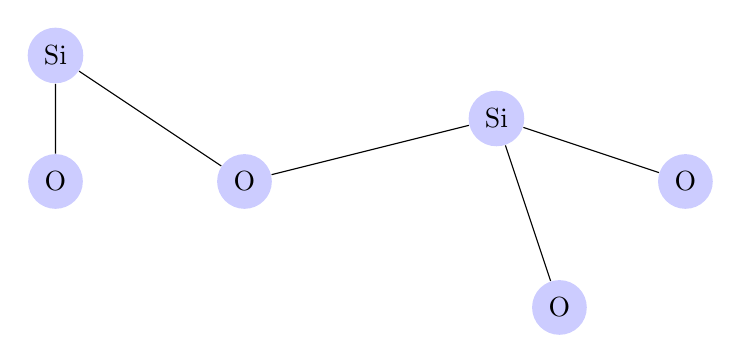
\begin{tikzpicture}
  [scale=.8,auto=left,every node/.style={circle,fill=blue!20}]
  \node (n6) at (1,10) {Si};
  \node (n4) at (4,8)  {O};
  \node (n5) at (8,9)  {Si};
  \node (n1) at (11,8) {O};
  \node (n2) at (9,6)  {O};
  \node (n7) at (1,8)  {O};

  \foreach \from/\to in {n6/n4,n4/n5,n5/n1,n2/n5,n6/n7}
    \draw (\from) -- (\to);

\end{tikzpicture}
\bigskip
\\
Due to the rapid nature of change within the molecular dyanmic simulations, there is one problem that must be address. The exploration of a single graph, or multi graph representation. This will be a challenge that we will have to investigate.   

\item \textbf{Method for Identifying Local Structures in the Graph}
\bigskip
\\
In order to predict where a fracture nucleates we must be able to identify any structures within the graph that might be associated with a fracture. Our above graph as we said was undirected and unweighted but if we look closer we can see associated structures. There are two molecules present in the graph, an $\ SiO_{3}$ and an $\ SiO_{2}$. Together they both share 1 oxygen atom, this is called a \textit{covalent} bond.
\bigskip
\\
Glasses containing nano-voids and atomic defects (such as under- and over-coordinated silicon and oxygen atoms) are less brittle than flaw-free bulk glasses. As fractures occur and propagate, there are more under- and over-coordinated silicon and oxygen atoms. We want to utilize this information as we utilize our adjacency matrix in our prediction on nucleation events. 
    \item \textbf{Stress Tensors:} We want to consider the direction in which the stress tensor is being applied. This has a direct affect on the size of a fracture and where it will emerge.
\end{itemize}

\begin{itemize} \item \textbf{Feature Extraction} 
\bigskip
\\
We plan to identify features of the graph network by using machine learning (ML) techniques. We aim to construct a ML algorithm that we will use to train data. This data is represented at time steps and will enable us to make predictions of where fractures will occur for later time steps. We will construct this graph using adjacency matrices.

To find features, we want to examine the relationship between nodes and fractures, which we may do so using the radial distribution function (RDF) or the k-nearest neighbors algorithm (KNN). Doing so will allow us to identify the smallest distance nodes may be within one anther before a fracture emerges.
\bigskip
\\
\textbf{Radial Distribution Function:} The radial distribution function (RDF) measures the probability of a node existing at a given distance away from a specific particle. To construct this function we pick a node and draw a series of concentric circles around it at a fixed distance. The number of atoms found in each shell is counted and stored at periodic intervals. The average number of atoms in each shell is calculated at the end of the simulation. To get the RDF, that average is then divided by the volume of each shell and the average density of the atoms. We will use the RDF to examine node distance periodically throughout the simulations, specifically when fractures begin. The RDF is also known as a radial pair distribution function. We can use the Average Radial Distribution function or the site-specific radial distribution function. The former calculates between two groups of atoms while the latter takes as input a list of pairs of atomic groups and outputs a list of RDF's between specific atomic groups.
\bigskip
\\
\textbf{K-nearest Neighbor:} The K-nearest neighbor (KNN) classification can help us predict the borders of the fractures. We can pick a random node and implement the KNN. We can classify that node either as that it contributed to the fracture or it didn't contribute to the fracture. If the nodes are a certain distance away from each other, and a fracture exists, we would classify those nodes as having contributed to the fracture. The distance away that is required to contribute to the fracture is to be determined.
    

First, we plan to use the above extracted features to predict fracture nucleation from a initial structure with no fracture. Additionally, we want to examine damage, meaning how a fracture may lead to another fracture, and so on. In particular, can cracks be isolated and not contribute to any further damage? We aim to address this concern and more. Moreover, we want to implement alpha shape in order to analyze fracture orientation, then we will examine fracture velocity and fracture tips.

By examining these two features, we will be able to predict where an initial fracture may occur. We will then study the properties of this fracture to predict the future behavior of our structure.

To identify local structure, the 2017-2018 paper uses a Gaussian kernel to "convert distances to similarities" (page 5). Use this possibly? This paper also lists all the parameters and what they define the parameters to be.
\end{itemize}

\begin{itemize}
\item \textbf{Machine Learning Methods} 

The culminating purpose of this project is to produce a machine learning model based on supervised learning techniques. 


\end{itemize}



\section{Milestones}
\label{sec: Milestones}
\begin{enumerate}

\item { Graph representation implemented in Python.}
\item {Feature Extraction from the MD simulation data to create training set.} 
\item {Create ensemable classificaiton  as well as a recurrant neural network using Python packages such as sci-kit learn, Keras and Tensorflow.} 
\item {Feature analysis and fine tuning parameters for increased accuracy. } 
\item {Finalized surrogate model.}
        
\end{enumerate}












\section{Deliverables}
\label{sec: Deliverables}
\begin{enumerate}
\item Graph representation implemented in Python. 
\item Local structures identified and labled. 
\item Features extracted from graph and local structures.
\item Midyear presentation.
\item Midyear report. 
\item Machine Learning Model Produced
\item Model validated on existing test sets.  
\item Journal article on our graph-theortic ML approaches.
\item Final presentation
\item Final Report

\end{enumerate}


\section{Schedule}
\label{sec: Schedule}
\begin{tabular}{ l|l } 
 \hline
 Date & Description  \\
 \hline
 November 20, 2019 & Midyear Presentation at CGU   \\ 
 December 20, 2019 & Midyear Report \\ 
 May 5, 2020 & Final Presentation at CGU \\ 
 May 12, 2020 & Completion of Project \\ 
 TBD & Site Visit and Presentation at Sandia National Laboratory  \\ 
\end{tabular}\\


%%% Appendices.

%%% For your Statement of Work, you probably won't have any
%%% appendices, but you could include some if you really needed to.

%%% The appendices are delineated with the \appendix command.
%%% Individual appendices are begun with the standard \chapter or
%%% \section commands.  In our example, we'll \include them just as we
%%% did other chapters.

%%% Even in a relatively short document such as your statement of
%%% work, you might need to have appendices.  If so, uncomment
%%% the \appendix command and add them below (remember, the
%%% top-level structural command in this format is section).

% \appendix


%%% Bibliography.

%%% BibTeX is the tool to use for citations and layout of your
%%% bibliography.  Instead of having to type ``[5]'' or ``(Jones,
%%% 1968)'' (and keep track of which citation is which and renumber
%%% them as you add more references to your bibilography), you use
%%% special commands that allow BibTeX and LaTeX to automatically put
%%% the correct information in the right place.

%%% Section 5.6 in _The Mathematics Clinic in Brief: A Handbook_,
%%% talks about using BibTeX to format your bibliography and
%%% citations.

%%% Depending on your field, it may or may not be appropriate to list
%%% references for which you haven't included specific citations.  If
%%% your field sanctions such practices, or if you just want to get an
%%% idea of what you have in your bibliography file, you can include
%%% everything with the \nocite{*} command.          

%%% The appearance of your bibliography and citations in your text are
%%% defined by a combination of any bibliography-related LaTeX
%%% packages (such as natbib, harvard, or chicago) and the particular
%%% bibliography style file that you load with the \bibliographystyle
%%% command.  Bibliography-style files end in .bst; you can find them
%%% by searching your file system using whatever tools you have for
%%% doing searches.  (On most modern Unices, ``locate .bst'' will give
%%% you an idea of what's available.)

%%%%\bibliographystyle{IEEEtran}

%%% The particular bibliography data file or files that you want to
%%% use are specified with the \bibliography file.  Multiple files are
%%% separated by commas.

%%% You might want to use multiple bibliography (or ``bib'') files if
%%% you had a master bib file containing references you use again and
%%% again, and another containing only records for references for a
%%% particular project.

%%% Many people create a single, large bib file that they use for
%%% everything they write.  That approach requires you to \cite every
%%% reference that you want to use in your document -- using
%%% \nocite{*} with a huge bibliography database will give you a large
`%%% bibliography containing many references you haven't consulted for
%%% your particular document!
\bibliographystyle{IEEEtran}
\small
%\nocite{*}
\bibliography{Bibliography}


%%% Glossary or Index.

%%% Having a glossary or index in a statement of work is overkill.
%%% Just define your terms in the text and you'll be fine.

\end{document}


